\documentclass [a4paper,11pt]{article}
\usepackage{booktabs}
\usepackage{zhfontcfg}
\usepackage{multirow}
\usepackage[margin=1in]{geometry}


\title{顺序图}
\date{\today}
\author{LetsGo安卓应用开发小组}

\begin{document}
	
\maketitle
\section*{修订历史}

\begin{table}[!hbp]
\centering

\begin{tabular*}{\textwidth}{c|c|c|c}
\hline
\rule{0pt}{0.8cm}
版~本 & 日~期 & 描~述 & 作~者\\
\hline
\rule{0pt}{0.6cm}
初始草案 & 2014年5月10日 & 第一个草案。主要进行细化以及精化。 & 王旸\\
\hline
\rule{0pt}{0.6cm}
 &  &  & \\
\hline
\end{tabular*}
\end{table}


\section*{顺序图}	
\subsection*{Planning过程顺序图}
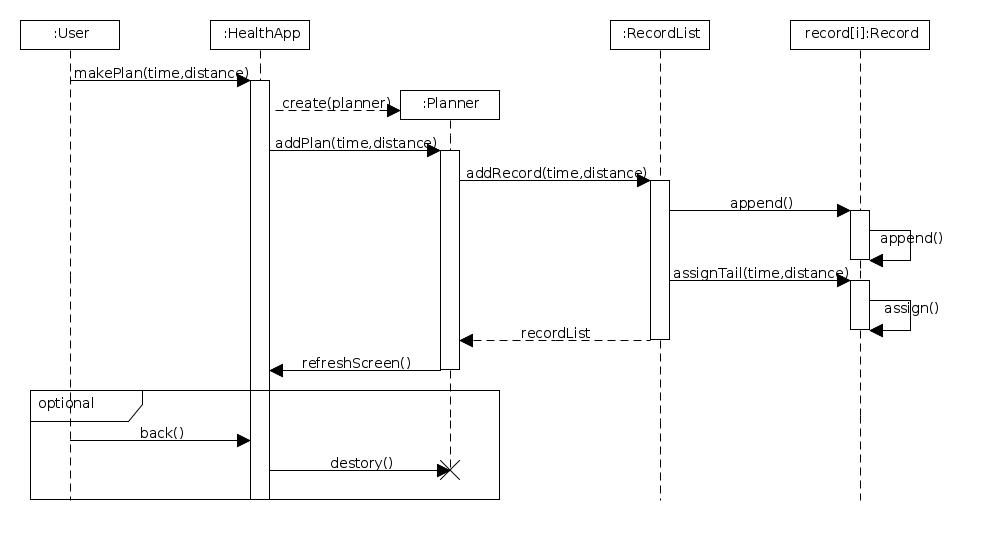
\includegraphics[width=\textwidth]{../SequenceDiagram_Planning.png}
\subsection*{Recording过程顺序图}
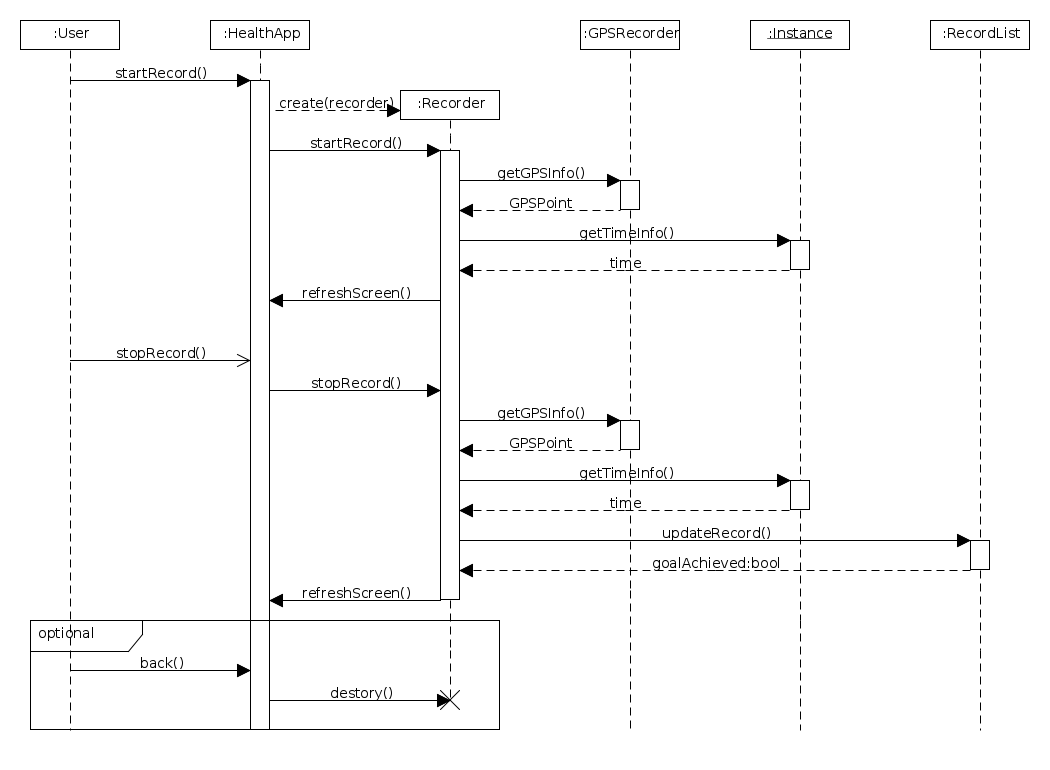
\includegraphics[width=\textwidth]{../SequenceDiagram_Recording.png}
\subsection*{Viewing过程顺序图}
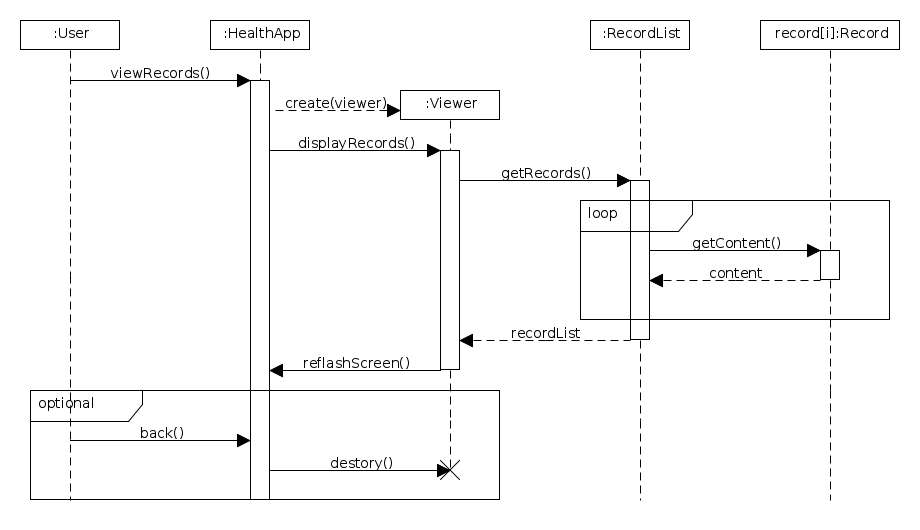
\includegraphics[width=\textwidth]{../SequenceDiagram_Viewing.png}

  
\end{document}
